% Emacs settings: -*-mode: latex; TeX-master: "manual.tex"; -*-

\chapter{Beam optical components:
Arms, slits, filters etc.}
This chapter contains a number of optical components
that is used to modify the neutron beam in various ways,
as well as the ``generic'' component \textbf{Arm}.
\index{Library!Components!optics}
\index{Optics|textbf}

\section{Arm: The generic component}
\label{s:arm}
\index{Optics!Point in space (Arm, Optical bench)}
\mcdoccomp{optics/Arm.parms}


The component \textbf{Arm} is empty; is resembles an optical bench
and has no effect on the xray.
The purpose of this component is only to provide a standard
means of defining a local coordinate system within the instrument definition.
Other components may then be
positioned relative to the \textbf{Arm} component
using the \MCX\ meta-language.
The use of \texttt{Arm} components in the instrument definitions
is not required but is recommended for clarity.
\textbf{Arm} has no input parameters.

The first Arm instance in an instrument definition may be changed into a
\verb+Progress_bar+(sec.~\ref{s:progress_bar}) component in order to display
simulation progress on the fly , and possibly save intermediate results.


\section{Slit: A beam defining diaphragm}
\label{slit}
\index{Optics!Slit}

%\component{Slit}{System}{$x_{\rm min}$, $x_{\rm max}$, $y_{\rm min}$, $y_{\rm max}$}{$r$, $p_{\rm cut}$}{}
\mcdoccomp{optics/Slit.parms}

The component {\bf Slit} is a very simple construction.
It sets up an opening at $z=0$, and propagates the neutrons
onto this plane (by the kernel call PROP\_Z0).
Neutrons within the slit opening are unaffected,
while all other neutrons
are discarded by the kernel call ABSORB.

By using {\rm Slit}, some neutrons contributing to the background
in a real experiment will be neglected.
These are the ones that scatter off the inner side
of the slit, penetrates the slit material,
or clear the outer edges of the slit.

The input parameters of {\bf Slit} are the four coordinates,
$(x_{\rm min}, x_{\rm max}, y_{\rm min}, y_{\rm max})$
defining the opening of the rectangle, or the radius $r$ of
a circular opening, depending on which parameters are specified.

The slit component can also be used to discard insignificant 
({\em i.e.}\ very low weight)
neutron rays, that in some simulations may be very abundant and therefore
time consuming. If the optional parameter $p_{\rm cut}$ is set, all
neutron rays with $p<p_{\rm cut}$ are ABSORB'ed.
This use is recommended in connection with {\bf Virtual\_output}.




\section{Slit\_N: multiple slits}
\label{s:slit-n}
\mcdoccomp{optics/Slit_N.parms}

Documentation pending.


\section{Beamstop: A photon absorbing area}
\label{beamstop}
\index{Optics!Beam stop}

\mcdoccomp{optics/Beamstop.parms}

The component \textbf{Beamstop} can be seen as the reverse of
the \textbf{Slit} component.
It sets up an area at the $z=0$ plane. Photons that hit the plane 
within this area are ABSORB'ed, while all others are unaffected.

By using this component, some photons contributing to the background
in a real experiment will be neglected.
These are the ones that scatter off the side
of the (real) beamstop, or penetrate the absorbing material.
Further, the holder of the beamstop is not simulated.

\textbf{Beamstop} can be either circular or rectangular.
The input parameters of \textbf{Beamstop} are either height and width $(x_{width},y_{height})$ or the four coordinates,
$(x_\mathrm{min}, x_\mathrm{max}, y_\mathrm{min}, y_\mathrm{max})$
defining the opening of a rectangle, or the radius $r$ of
a circle, depending on which parameters are specified.

If the "direct beam" (e.g. after a monochromator or sample) should not be
simulated, it is possible to emulate an ideal beamstop 
so that only the scattered beam is left;
without the use of \textbf{Beamstop}:
This method is useful for instance in the case where only photons 
scattered from a sample are of interest. 
The example below removes the direct beam and 
any background signal from other parts of the instrument
\begin{verbatim}
COMPONENT MySample=V_sample(...) AT (...)
EXTEND
%{
  if (!SCATTERED) ABSORB;
%}
\end{verbatim}


\section{Filter: A general absorption filter model}
\label{s:filter}
\index{Optics!Filter}
\mcdoccomp{optics/Filter.parms}

This component is a filter in the shape of a rectangular block or a general
shape defined by a set of polygons. Given an input file containing material
parameters. Neccessary parameters are nominal density and a parameterization of
the linear attenuation coefficient, $\mu$ as a function of wavelength (or
energy).

The model is very simple: Firstly the X-ray is traced to find intersection points between ray and filter (0 or 2).
If no intersection is found the x-ray is left untouched and nothing further happens.
Assuming the ray intersects the filter: Secondly, the path length d$l$ within the filter is computed.
Thirdly a $\mu = f(\lambda,\mathrm{material})$ is computed by interpolating in
a datafile, and the x-ray weight is adjusted according to
$p=p\exp(-\mathrm{d}l*\mu)$. The x-ray is left at the point where it exits the
filter block (the $2$nd intersection).

Example data files corresponding to all elements up to $Z=92$ are distributed with \MCX in the
\verb+MCXTRACE/data+ directory as \verb+*.txt+ files. These tables have been
extracted from the NIST FFAST~\cite{NIST-ffast} x-ray database.
To generate other datafiles from the same source a simple shell script:
\verb+MCXTRACE/data/get_xray_db_data+ is also distributed with \MCX
Running this script will connect to the NIST webiste and download a
\verb+.html+ file. This output must now be modified such that \verb+html+-tags
are removed and all header lines begin with $\#$

\subsection{Example}
\label{getNISTdata}
This is an example of how to download and generate datafiles for the \verb+Filter.comp+ and others.

The distributed tables have been extracted from the NIST x-ray database. To ease generation of more dtafiles
from the same source a simple shell script:\\
\verb+MCXTRACE/data/get_xray_db_data+\\
is also distributed with \MCX

Running this script will connect to the NIST webiste and download a \verb+.html+ file. This output must now be modified wuch that \verb+html+-tags
are removed and all header lines begin with $\#$.

\begin {verbatim}
 /usr/local/lib/mcxtrace/data/get_xray_db_data 3 output.dat
\end{verbatim}
where the second parameter (3) is the atom number of the material, for which we want to generate a datafile.
Now open the generated datafile (\verb+output.dat+) with your favourite text editor and make sure the file ends up looking like this
\tiny
\begin{verbatim}
#Li (Z 3)
#Atomic weight: A[r]  6.941000
#Nominal density: rho 5.3300E-01
#    σ[a](barns/atom) = [μ/ρ](cm^2 g^-1)  ×  1.15258E+01
#    E(eV) [μ/ρ](cm^2 g^-1) = f[2](e atom^-1)  ×  6.06257E+06
#    2 edges. Edge energies (keV):
#
#
#    K      5.47500E-02  L I    5.34000E-03
#
#Relativistic correction estimate f[rel] (H82,3/5CL) = -9.8613E-04,
#    -6.0000E-04 e atom^-1
#    Nuclear Thomson correction f[NT] = -7.1131E-04 e atom^-1
#
#━━━━━━━━━━━━━━━━━━━━━━━━━━━━━━━━━━━━━━━━━━━━━━━━━━━━━━━━━━━━━━━━━━━━━━━━━━━━━━━
#Form Factors, Attenuation and Scattering Cross-sections
#Z=3, E = 0.001 - 433 keV
#
#    E        f[1]         f[2]        [mu/rho]    [sigma/rho]  [mu/rho]   [mu/rho][K] lambda
#                                    Photoelectric Coh+inc      Total
#   keV        e atom^-1    e atom^-1   cm^2 g^-1   cm^2 g^-1   cm^2 g^-1   cm^2 g^-1  nm
5.233200E-03  9.08733E-01  0.0000E+00  0.0000E+00  2.3914E-07  2.3914E-07  0.000E+00  2.369E+02
5.313300E-03  8.59283E-01  0.0000E+00  0.0000E+00  2.5404E-07  2.5404E-07  0.000E+00  2.333E+02
5.334660E-03  8.03599E-01  0.0000E+00  0.0000E+00  2.5813E-07  2.5813E-07  0.000E+00  2.324E+02
5.366700E-03  8.56971E-01  1.0769E-01  1.2165E+05  2.6435E-07  1.2165E+05  0.000E+00  2.310E+02
.
.
.
3.788588E+02  3.00000E+00  3.9121E-08  6.2602E-07  8.4389E-02  8.4390E-02  6.123E-07  3.273E-03
4.050001E+02  3.00000E+00  3.3438E-08  5.0054E-07  8.2127E-02  8.2128E-02  4.895E-07  3.061E-03
4.329451E+02  3.00000E+00  2.8581E-08  4.0022E-07  7.9892E-02  7.9892E-02  3.913E-07  2.864E-03
\end{verbatim}
\normalsize
Please make sure you don't forget to remove the html-tags in the bottom of the file as well. In the future we will set
up a more streamlined way of doing this.


\section{Chopper\_simple: An ideal chopper}
\index{Optics!lens}
\mcdoccomp{optics/Chopper_simple.parms}

\texttt{Chopper\_simple} models a chopper by a blocking mathematical plane which becomes transparent'
in the specified time interval. 



\newpage
\chapter{Reflecting optical components: mirrors, and guides}
\index{Optics|textbf}
\section{Lens\_parab: an x-ray lens of a parabolic profile; could extend to many lenses, forming a compound refractive lens (CRL)}
\label{lens-parab}
\index{Optics!Lens\_parab}

An X-ray refractive lens, often referred to as a Compund Refractive Lens (CRL), is a fairly new type of device, which has gained popularity in
the last few years. An early study showing the feasiblity of such devices may be found in~\cite{snigirev1996}. As the refractive index of X-rays
is $n\approx1$ a number of lenses, stacked together is usually necessary to bring the focal length to practical values. 
\MCX includes a few lens components, which all have slightly different charactertics.


\section{Lens\_simple: Thin lens approximation}
\index{Optics!lens}

\mcdoccomp{optics/Lens_simple.parms}

This models a thin-lens approximation of a stack of parabolic refractive x-ray lenses

\section{Lens\_parab: Thick parabolic CRL}
\index{Optics!lens}
\mcdoccomp{optics/Lens_parab.parms}

Component model of a stack of compund refractive lenses. Each lens in the stack is modelled by two parabolic surfaces, and rays are traced through all the complete stack  taking the displace,ement of the surfaces into account. This is naturally less efficient than a thin lens approximation.

The functionality of \texttt{Lens\_parab\_Cyl}, \texttt{Lens\_parab\_rough}, and \texttt{Lens\_parab\_Cyl\_rough} will be merged into this component.

\section{Lens\_parab\_Cyl: Thick 1D-parabolic CRL}
\index{Optics!lens}
\mcdoccomp{optics/Lens_parab_Cyl.parms}

This component and its functionality is scheduled to be merged into \texttt{Lens\_parab}


\section{Lens\_parab\_rough: Thick parabolic CRL including roughness-model}
\index{Optics!lens}
\mcdoccomp{Lens_parab_rough.parms}

This component and its functionality is scheduled to be merged into \texttt{Lens\_parab}

\section{Lens\_parab\_Cyl\_rough: Thick 1D-parabolic CRL including roughness-model}
\label{s:lens-parab-cyl-rough}
\index{Optics!lens}
\mcdoccomp{optics/Lens_parab_Cyl_rough.parms}

Identical to \textbf{Lens\_parab\_Cyl} except it has the option of a \textit{roughness} parameter.
Roughness is simply modelled by a stochatstic, normally distributed, displacement of the normal vector of the lens surfaces.

This component and its functionality is scheduled to be merged into \texttt{Lens\_parab}


\section{Lens\_Kinoform: refractice kinoform lens}
\index{Optics!lens}
\mcdoccomp{optics/Lens_Kinoform.parms}

Doc. Pend.

\section{Lens\_elliptical: }
\index{Optics!lens}
\mcdoccomp{Lens_elliptical.parms}

doc. pend.




\index{Optics|textbf}

This section describes advanced X-ray optics
components such as mirrors and analyzer crystals.
A description of the reflectivity of a mirror is found
in section~\ref{ss:mirrorreflect}.

\section{Mulitlayer\_elliptic: The elliptic multilayer mirror}
\label{s:mirror}
\index{Optics!Mirror plane}
\component{Multilayer\_elliptic}{System}{$\theta$, $s1$, $s2$, $length$, $width$, $R$}{}{validated}
%{$R_0, Q_c, W, \alpha, reflect$}{validated}

The component \textbf{Multilayer\_elliptic}
models a single rectangular reflecting multilayer mirror plate with elliptical curvature. It can be used
as a sample component, to \textit{e.g.}~assemble a Kirkpatrick-Baez focusing system 
or in combination with a double-crystal monochromator.


Figure~\ref{fig:Ellipse}\emph{Left} shows a side view of a mirror
(the blue section of the ellipse) in the McXtrace coordinate system.
At the mirror center, the mirror tangent is parallel to the $z$ axis
and the mirror normal is parallel to the $y$ axis. The width of the
mirror is $w$ and in $y-z$ plane the mirror has the curvature of an
ellipse with major axis $a$ and minor axis $b$,
%
\begin{equation} 
\frac{z^2}{ a^2} + \frac{y^2}{b^2} =1\,, \,|x| <
\frac{w}{2}\,.
\end{equation}
%
The length of the mirror is $L$. The coordinates of the mirror
center $(0,Y_0,Z_0)$ and the ellipse parameters $a$, $b$ are
determined uniquely by the central glancing angle, the source-mirror
distance and the mirror-image distance. The position of the mirror
is chosen to be at the positive side of the $y$ axis.

The input parameters of this component are:
$\theta$ [$^{\circ}$], the incident angle; 
$s1$ [m], the distance from the source to the multilayer;
$s2$ [m], the focusing distance of the multilayer;
$length$ [m], the length of the mirrors;
$width$ [m], the width of the mirror along the $x$-axis;
$R$, the reflectivity.

\subsection{Definition of the reference frames}
The direction and position of the incoming photon is defined
relative to the coordinate system illustrated in
Fig.~\ref{fig:Ellipse}\emph{Left} (in the code referred to as
\emph{McXtrace coordinate system}):
\begin{itemize}
\item the y-axis is parallel to the central mirror normal
\item the z-axis is parallel to the central mirror tangent
\item the origin is at the mirror center
\end{itemize}

However, all the calculations are conducted in another reference
frame which is illustrated in Fig.~\ref{fig:Ellipse}~\emph{Right}(in
the following referred to as the \emph{Ellipse coordinate system}):
\begin{itemize}
\item the z-axis is parallel to major axis of ellipse
\item the y-axis is parallel to minor axis of ellipse
\item the origin is at the center of the ellipse
\item the mirror center at $(0,Y_0,Z_0)$, uniquely determined by the
glancing angle at the mirror center, the source-mirror distance and
mirror-image distance.
\end{itemize}

\begin{figure}[htb!]
\centering
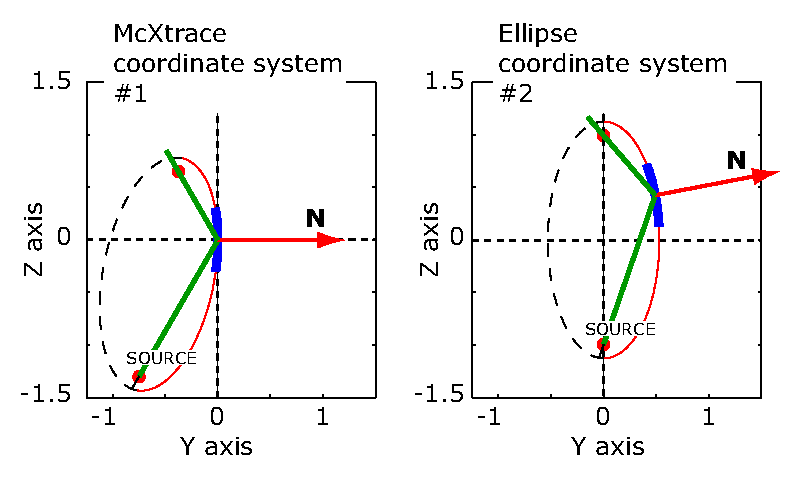
\includegraphics[width=0.95\linewidth]{figures/ellipse.eps}
 \caption{The same image in different coordinate systems.\newline \emph{Left}:
 \emph{McXtrace System} with the y-axis is parallel to the central mirror normal, the z-axis
 is parallel to the central mirror tangent and the origin is at the mirror
 center. \newline
 \emph{Right}: \emph{Ellipse System} with
the z-axis parallel to major axis of ellipse, the y-axis is parallel
to minor axis of ellipse and the origin is at the center of the
ellipse. }\label{fig:Ellipse}
\end{figure}


\subsection{Algorithm}
\begin{enumerate}
\item The photon is generated with a starting point $\bf{S}$ and a direction
$\bf{V}_\textrm{in}$ defined in the \emph{McXtrace} coordinate
system.
\item All calculations are performed in the \emph{Ellipse} coordinate system,
so to proceed the basis is changed to that reference frame.
\item The 2 intersections of the ray with the ellipse are determined.
\item It is checked if any of the intersections are within the area
defined by the mirror.
\item If one of the solutions is valid, the reflection of that ray is
determined.
\item The coordinates of the starting point and direction of the
reflected ray are calculated using the basis of the \emph{McXtrace}
coordinate system.
\end{enumerate}


\section{Reflection of the ray in the mirror}
\begin{figure}[htb!]
\centering
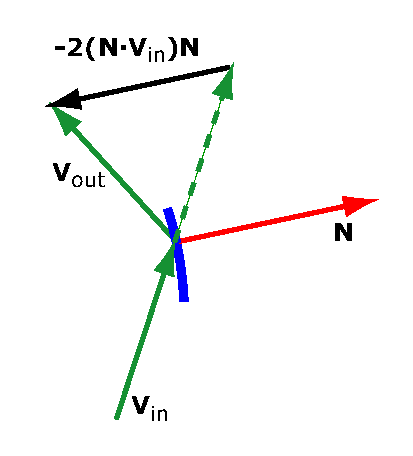
\includegraphics[width=0.3\linewidth]{figures/Dotproduct.eps}
 \caption{The reflection of the unit vector $\bf{V}_\textrm{in}$ in the mirror with the normal unit
 vector $\boldsymbol{{N}}$ is $\boldsymbol{{V}}_\textrm{out} = \boldsymbol{{V}}_\textrm{in} -2(\boldsymbol{{N}}\cdot\boldsymbol{{V}}_\textrm{in})\boldsymbol{{N}}$}\label{fig:dotProduct}
\end{figure}

The tangent and normal to the ellipse $z^2/a^2 + y^2/b^2=1$ at the
point $(Y,Z)$ are found by implicit differentiation: \begin{equation} 
\frac{2z}{a^2} + \frac{2y}{b^2} \,\frac{dy}{dz} = 0\,, \end{equation} so at the
point $(Y,Z)$ the slope of the tangent is $\frac{dy}{dz} =
-\frac{Z\,b^2}{Y\,a^2}$. The slope of the normal is minus the
inverse of the tangent slope, so the coordinates of the mirror
normal are \begin{equation} N_x = 0 \quad N_y = \frac{a^2\,Y}{b^2\,Z} \quad N_z =
1\,. \end{equation} With $\bf{V}_\textrm{in}$ and $\bf{N}$ denoting unit
vectors (direction and normal respectively), the direction of the
reflected ray is calculated as \begin{equation} \boldsymbol{{V}}_\textrm{out} =
\boldsymbol{{V}}_\textrm{in} -2(\boldsymbol{{N}}\cdot\boldsymbol{{V}}_\textrm{in})\boldsymbol{{N}} =
        \left(
      \begin{array}{c}
        V_{\textrm{in}x} - 2(\boldsymbol{{N}}\cdot\boldsymbol{{V}}_\textrm{in})N_x \\
               V_{\textrm{in}y} - 2(\boldsymbol{{N}}\cdot\boldsymbol{{V}}_\textrm{in})N_y \\
                V_{\textrm{in}z} - 2(\boldsymbol{{N}}\cdot\boldsymbol{{V}}_\textrm{in})N_z \\
      \end{array}
    \right)
\end{equation}


\subsection{Mirror reflectivity}
\label{ss:mirrorreflecttable}

At present, the Multilayer\_elliptic Mirror component uses a reflectivity table $reflect$, 
which 1st column is q [$\AA^{-1}$] and from the 2nd column on as the reflectivity $R$ in [0-1]
as function of tabulated energy [$KeV$]. 
An example file, calculated for a particular $Si/W$ multilayer, is provided (\verb+reflectivity.txt+).
User provided reflectivity data files can be parsed by the component.



\section{Mirror\_curved}
\label{mirror-curved}
\index{Mirror!Cylindrically curved mirror}
\component{Mirror\_curved}{System}{\textit{radius,length,width}}{\textit{coating,R0}}{}
 
Models a cylindrical mirror, positioned in the XZ-plane curving towards
positive X. The input parameter \textit{radius} defines the radius of curvature
and the mirror size is given by \textit{length} and \textit{width} where length
and width is along Z and Y respectively. $coating$ and $R0$ are mutually
exclusive. If \textit{R0} is nonzero, it is taken as the reflectivity value,
irrespective of wavelength, whereas coating nominates a file from which to read
values for $f_1$ and $f_2$. See~\cite{NIST-ffast} for definitions. For
elements $Z\in[1,92]$ datafiles are distributed with the McXtrace system that
may be used as: \verb+coating="Rh.txt"+. or \verb+coating="Al.txt"+. 

\section{Mirror\_curved: Cylindrically curved mirror}
\index{Optics!mirror}

\mcdoccomp{optics/Mirror_curved.parms}

Models a cylindrical mirror, positioned in the XZ-plane curving towards
positive X. The input parameter \textit{radius} defines the radius of curvature
and the mirror size is given by \textit{length} and \textit{width} where length
and width is along Z and Y respectively. \textit{coating} and \textit{R0} are mutually
exclusive. If \textit{R0} is nonzero, it is taken as the reflectivity value,
irrespective of wavelength, whereas coating nominates a file from which to read
values for $f_1$ and $f_2$. See~\cite{NIST-ffast} for definitions. For
elements $Z\in[1,92]$ datafiles are distributed with the McXtrace system that
may be used as: \verb+coating="Rh.txt"+. or \verb+coating="Al.txt"+. 

This component is scheduled to be merged with \texttt{Mirror\_parabolic} and \texttt{Mirror\_elliptic} 

\section{Mirror\_parabolic: Mirror with a parabolic curvature profile.}
\index{Optics!mirror}

\mcdoccomp{Mirror_parabolic.parms}

This component is scheduled to be merged with \texttt{Mirror\_elliptic}

\section{Mirror\_elliptic: Mirror with a elliptic curvature profile.}
\index{Optics!mirror}

\mcdoccomp{Mirror_elliptic.parms}

This component is scheduled to be merged with \texttt{Mirror\_parabolic}



\section{Multilayer\_elliptic: Elliptically curved mirror coated with a multilayer}
\index{Optics!multilayer, mirror}

\mcdoccomp{optics/Multilayer_elliptic.parms}

doc. pend.


\section{TwinKB\_ML: Side-by-side Kirkpatrick-Baez mirror pair}

\mcdoccomp{optics/TwinKB_ML.parms}

Models a pair of perpendicular, elliptically curved mirrors, known as a Montel-mirror or Side-by-side Kirkpatrick-Baez mirror.

